Thiết kế khái niệm là mức thiết kế đầu tiên của cơ sở dữ liệu. Ở mức này, hệ thống được mô tả dưới góc nhìn nghiệp vụ thông qua các thực thể, thuộc tính và mối quan hệ giữa các thực thể mà chưa phụ thuộc vào hệ quản trị cơ sở dữ liệu cụ thể.

\section{Xác định thực thể và thuộc tính}

Dựa trên yêu cầu nghiệp vụ, hệ thống gồm chín thực thể chính.

\begin{table}[htbp]
    \centering
    \caption{Thực thể và thuộc tính}
    \label{tab:entity_attributes}
    \begin{tabularx}{\textwidth}{|p{2.8cm}|p{5.5cm}|X|}
        \hline
        \textbf{Thực thể} &
        \textbf{Thuộc tính} &
        \textbf{Ý nghĩa} \\ \hline

        \textit{Customer} &
        customer\_id, full\_name, phone, email, address &
        Thông tin định danh và liên hệ của khách hàng. \\ \hline

        \textit{Pet} &
        pet\_id, name, species, breed, age, customer\_id &
        Thông tin cơ bản của thú cưng và khách hàng sở hữu. \\ \hline

        \textit{Veterinarian} &
        vet\_id, full\_name, schedule &
        Thông tin bác sĩ và lịch làm việc. \\ \hline

        \textit{Staff} &
        staff\_id, full\_name, role &
        Thông tin nhân viên hỗ trợ. \\ \hline

        \textit{Admin} &
        admin\_id, username, password &
        Thông tin tài khoản quản trị. \\ \hline

        \textit{Booking} &
        booking\_id, date\_time, status, payment, customer\_id, pet\_id, vet\_id, staff\_id &
        Thông tin lịch đặt khám và các đối tượng tham gia. \\ \hline

        \textit{Invoice} &
        invoice\_id, amount, date, status, booking\_id &
        Thông tin hóa đơn của một booking. \\ \hline

        \textit{MedicalRecord} &
        record\_id, diagnosis, treatment, date, pet\_id, vet\_id &
        Thông tin chẩn đoán và điều trị. \\ \hline

        \textit{Room} &
        room\_id, room\_type, status, note &
        Thông tin phòng chăm sóc. \\ \hline
    \end{tabularx}
\end{table}

\section{Xác định khóa chính}

Mỗi thực thể được xác định bởi một khóa chính duy nhất:

\begin{table}[htbp]
    \centering
    \caption{Khóa chính của các thực thể}
    \label{tab:primary_keys}
    \begin{tabular}{|p{3cm}|p{5cm}|}
        \hline
        \textbf{Thực thể} & \textbf{Khóa chính} \\ \hline
        Customer & customer\_id \\ \hline
        Pet & pet\_id \\ \hline
        Veterinarian & vet\_id \\ \hline
        Staff & staff\_id \\ \hline
        Admin & admin\_id \\ \hline
        Booking & booking\_id \\ \hline
        Invoice & invoice\_id \\ \hline
        MedicalRecord & record\_id \\ \hline
        Room & room\_id \\ \hline
    \end{tabular}
\end{table}

\section{Xác định mối quan hệ}

Các mối quan hệ giữa các thực thể được xác định như sau:

\begin{table}[htbp]
    \centering
    \caption{Các mối quan hệ giữa các thực thể}
    \label{tab:relationships}
    \begin{tabularx}{\textwidth}{|c|p{6cm}|X|}
        \hline
        \textbf{Quan hệ} &
        \textbf{Mô tả} &
        \textbf{Mối quan hệ} \\ \hline

        Customer -- Pet &
        Một khách hàng có thể sở hữu nhiều thú cưng. &
        1:N \\ \hline

        Customer -- Booking &
        Một khách hàng có thể tạo nhiều booking. &
        1:N \\ \hline

        Pet -- Booking &
        Một thú cưng có thể có nhiều booking. &
        1:N \\ \hline

        Veterinarian -- Booking &
        Một bác sĩ có thể phụ trách nhiều booking. &
        1:N \\ \hline

        Staff -- Booking &
        Một nhân viên có thể xử lý nhiều booking. &
        1:N \\ \hline

        Pet -- MedicalRecord &
        Một thú cưng có thể có nhiều hồ sơ khám. &
        1:N \\ \hline

        Veterinarian -- MedicalRecord &
        Một bác sĩ có thể tạo nhiều hồ sơ khám. &
        1:N \\ \hline

        Booking -- Invoice &
        Một booking có thể chưa có hoặc có tối đa một hóa đơn. &
        1:0..1 \\ \hline
    \end{tabularx}
\end{table}

\section{Mô hình ERD}

Từ các thực thể, thuộc tính và mối quan hệ đã xác định, mô hình ERD của hệ thống được xây dựng như hình dưới đây.

\begin{figure}[htbp]
    \centering
    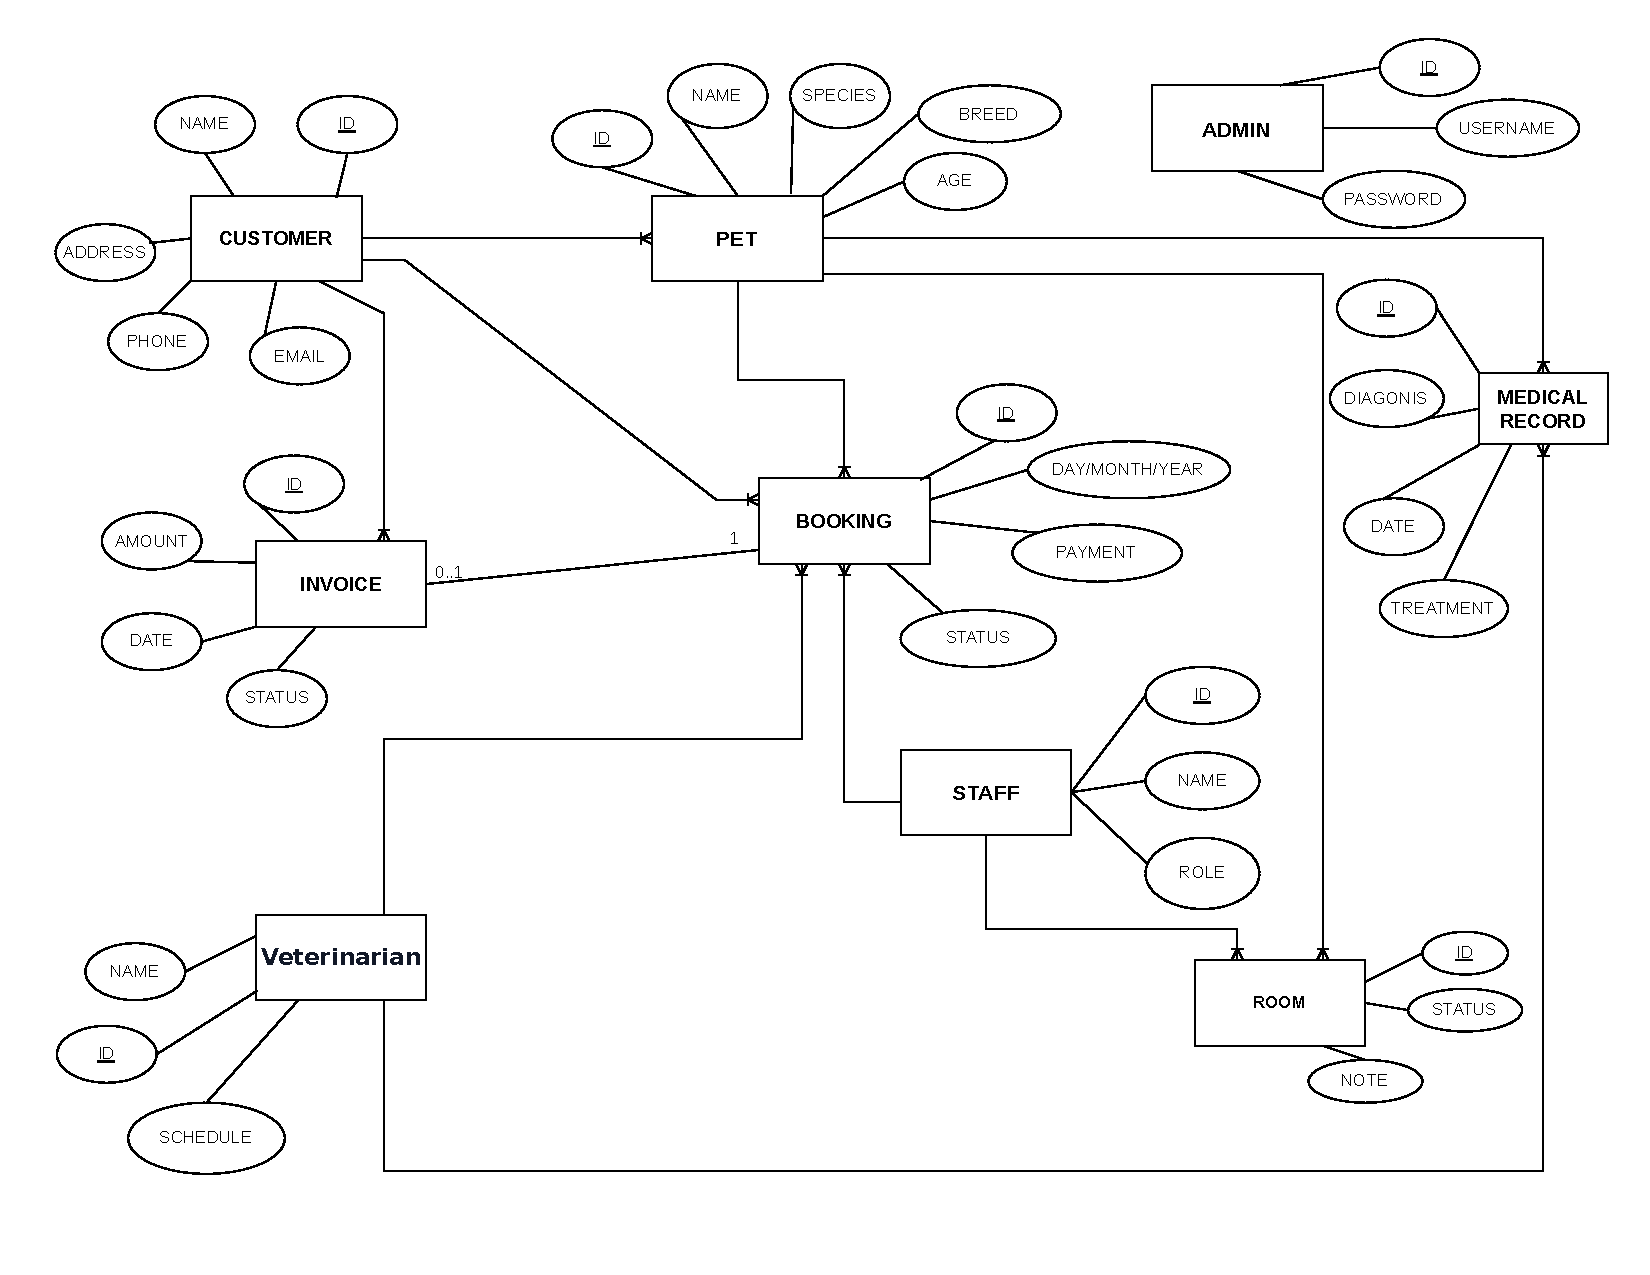
\includegraphics[
        width=\textwidth,
        height=0.8\textheight,
        keepaspectratio
    ]{figures/pet_health_care_erd.pdf}
    \caption{Mô hình ERD của hệ thống Chăm sóc Sức khỏe Thú cưng}
    \label{fig:pet_health_care_erd}
\end{figure}

\section{Kiểm tra mô hình khái niệm}

Mô hình ERD đáp ứng các yêu cầu nghiệp vụ chính của hệ thống. Các thực thể đều có khóa định danh riêng và các quan hệ đều thể hiện đúng số lượng bản ghi có thể tham gia.

Trong mô hình hiện tại không sử dụng thực thể yếu, không có quan hệ nhiều--nhiều và không sử dụng mô hình chuyên biệt hóa EER. Quan hệ Booking--Invoice được biểu diễn theo dạng một--không hoặc một.

\section{Kết luận chương}

Chương này đã hoàn thành mức thiết kế khái niệm thông qua việc xác định thực thể, thuộc tính, khóa chính, các mối quan hệ và mô hình ERD. Mô hình này sẽ được chuyển đổi sang mô hình quan hệ ở mức thiết kế logic.